%--------------------------------------------------------------------------------------
% Feladatkiiras (a tanszeken atveheto, kinyomtatott valtozat)
%--------------------------------------------------------------------------------------
% \chapter*{Feladatkiírás}
\phantomsection
\addcontentsline{toc}{chapter}{Feladatkiírás}

% A modern alacsony hőmérsékletű plazmafizikai kísérletek egy új, érdekes és izgalmas területe a poros plazmák
% kutatása. Egy elektromos gázkisülésbe helyezett apró (mikrométer méretű) szilárd szemcse a kisülési plazma
% atomi részecskéivel kölcsönhatva elektromosan feltöltődik. A sok töltött szemcséből kialakuló elrendezésben a
% szilárdtestfizikai jelenségek széles spektruma figyelhető meg, pl. kristályrács kialakulása, fázisátalakulás,
% diszlokációk dinamikája, transzport folyamatok, stb. Poros plazmákat jelenleg leginkább alapkutatásokban
% alkalmaznak, de jelentőségük az elektronikai gyártásban, fúziós
% reaktorok üzemeltelésében, {\color{red} terahertz}
% technológiában egyre inkább előtérbe kerül.
% 
% A kísérleti adatgyűjtés és feldolgozás nagyrésze részecske-követő velocimetrián (particle tracking velocimetry)
% alapul, vagyis első lépésben egy nagysebességű kamera segítségével nagyfelbontású képek készülnek, amely
% képek segítségével a porszemcsék pontos (a kamera felbontásánál pontosabb) koordinátáit kell meghatározni. A
% képek elemzése ezidáig csak a mérést követően, hosszú idő alatt volt megvalósítható a vizsgálandó nagy
% adatmennyiség miatt. A multiprocesszoros környezetek segítségével a feldolgozás gyorsítása lehetséges akár
% több nagyságrenddel is.
% 
% A jelölt feladata, hogy a meglévő kísérleti elrendezés, amely az MTA Wigner Fizikai Kutatóközpont
% Szilárdtestfizikai és Optikai Intézezetben található, kiegészítésével a mérés közbeni feldolgozással a mérést
% segítő analízist hajtson végre. Ennek eredményével a mérés előkészítése és elvégzése lényegesen gyorsulhatnak.
% 
% \begin{flushleft}
% \textbf{A jelölt feladata}
% 
% \begin{itemize}
% 	\item Mutassa be a mérési elrendezést és elemezze a kapott adatokat! (Mutassa
% 	be a mérést!)
% 	\item Elemezze a lehetséges multiprocesszoros környezeteket, a feladat
% 	szempontjából lényeges paraméterek és feladatvégrehajtási elvárások szempontjából!
% 	\item Készítsen programot, amely az azonnali (valós idejű) analízisben résztvevő paramétereket számítja ki, a
% 	multiprocesszoros környezet kihasználása nélkül!
% 	\item Készítsen programot, amely a mérési környezetbe illeszkedve a mérésnél
% 	valós időben képes a vizsgált paraméterek megjelenítésére! Mutassa be és
% 	elemezze az elkészített programot!
% 	\item Hasonlítsa össze a multiprocesszoros és a nem-multiprocesszoros
% 	környezetre elkészített programokat erőforrás igény illetve egyéb paraméterek szempontjából!
% \end{itemize}
% \end{flushleft}
% 
% \begin{flushleft}
% \textbf{Irodalom}:
% \begin{itemize}
% 	\item \cite{Hartmann2010} Hartmann P, et. al. ; “Crystallization Dynamics of a Single Layer Complex Plasma”;
% 	Phys. Rev. Lett., 105 (2010) 115004
% 	\item \cite{Hartmann2013} Hartmann P, et. al. ; “Magnetoplasmons in Rotating Dusty	Plasmas”, Phys.	Rev. Lett.
% 	111, 155002 (2013)
% 	\item \cite{HartmannP2013} Hartmann P, Donkó I, Donkó Z; “Single exposure three-dimensional imaging of dusty
% 	plasma clusters”; Rev. Sci. Instrum., 84 (2013) 023501/1-5;
% \end{itemize}
% \end{flushleft}
% 
% \begin{flushleft}
% \vspace*{1cm}
% \textbf{Tanszéki konzulens}: Reichardt András, egy. tanársegéd\\
% \textbf{Külső konzulens}: Hartmann Péter, PhD., tud. főmunkatárs (MTA Wigner FK, SZFKI)
% \end{flushleft}
% 
% 
% 
% \begin{flushleft}
% \vspace*{1cm}
% Budapest, 2014.03.10.
% \end{flushleft}

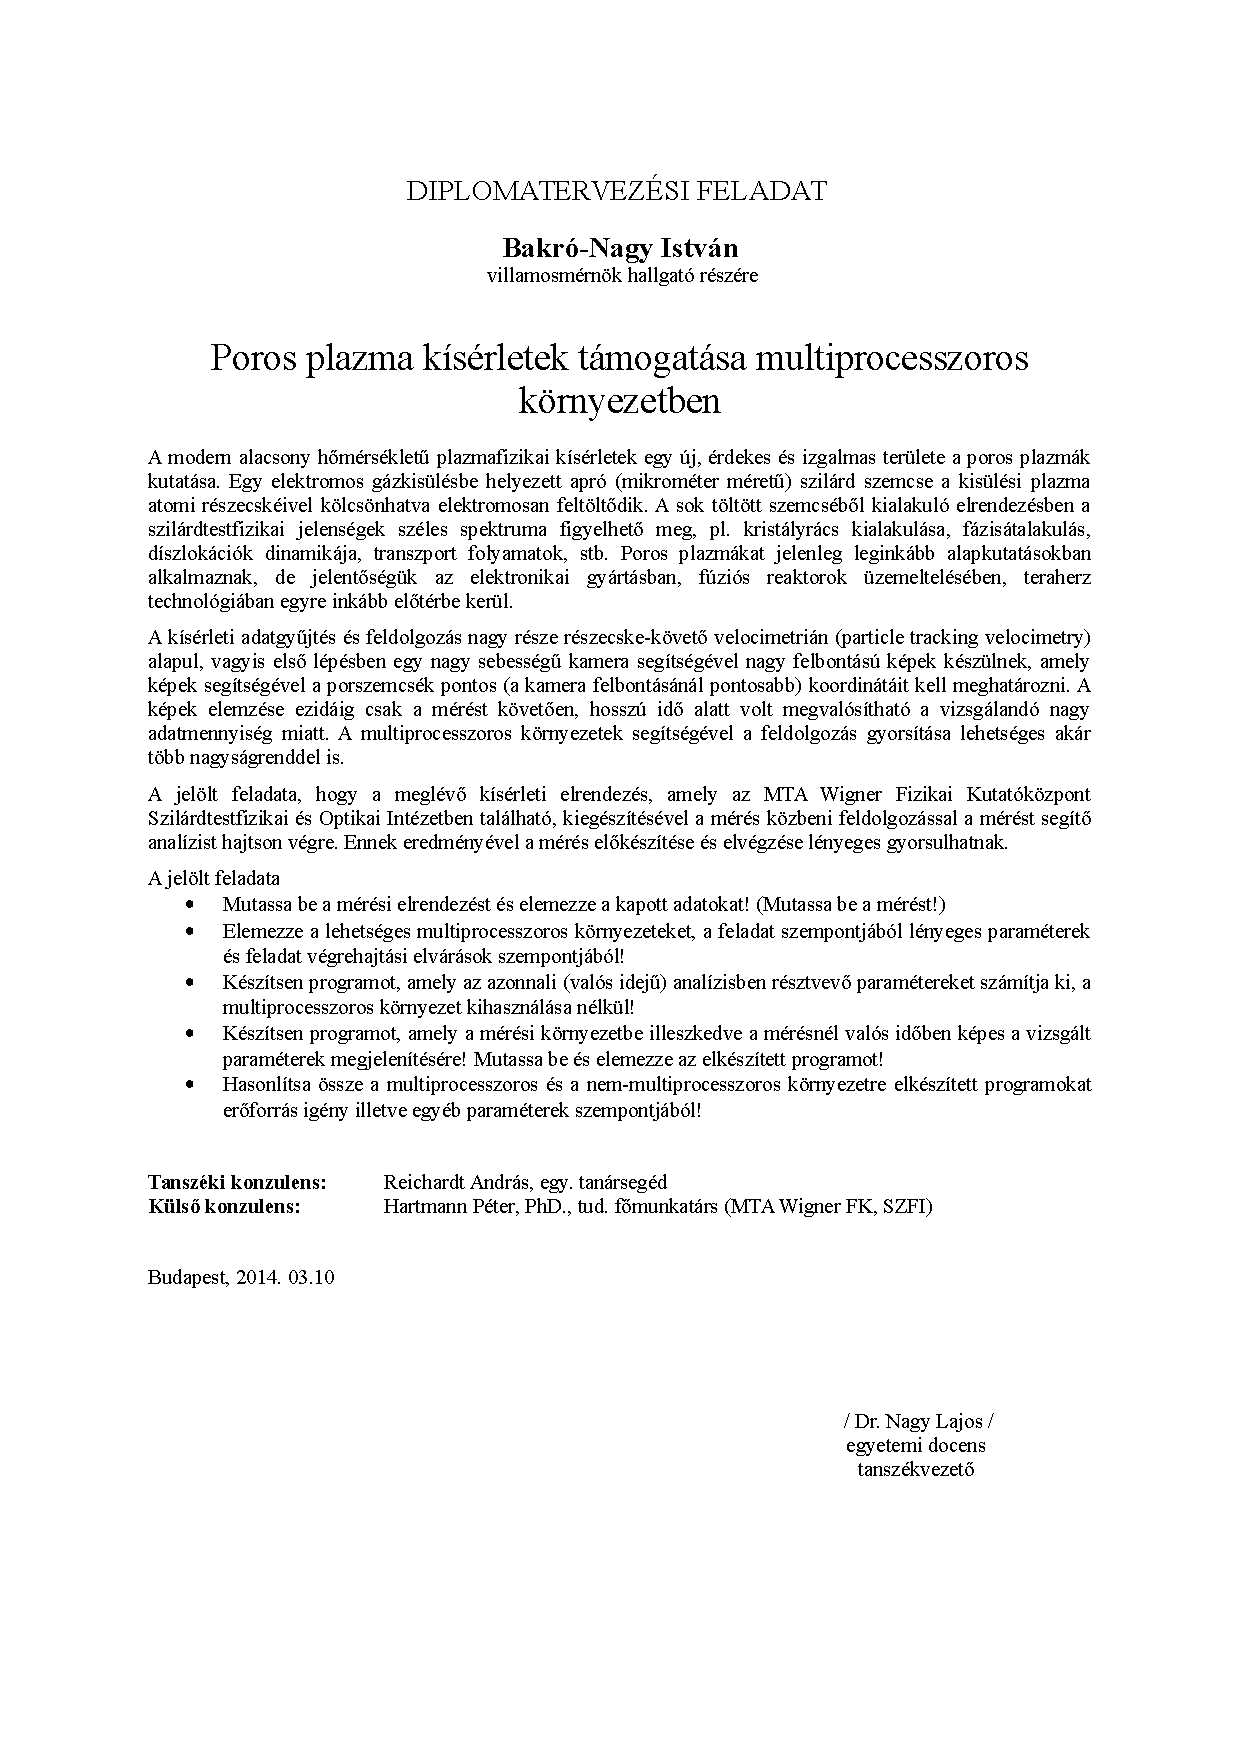
\includepdf[pages={1}]{kiiras.pdf}
